\documentclass[]{scrartcl}

\title{MIPS Home Computer System}
\subtitle{System Design Reference}
\author{
    \large Student\\
    \large Mostafa Abd El-Aziz\\
    \and
    \large Supervisor\\
    \large Prof. Dr. Layla Abou Hadid\\
}
\date{\vspace{-5ex}}

% font
\usepackage[T1]{fontenc}
\usepackage{lmodern}
\renewcommand*\familydefault{clms}
\usepackage{sfmath}
\usepackage{microtype}
\usepackage[utf8]{inputenc}
\usepackage{cfr-lm} % font package

% listings
\usepackage{listings}
\lstset{language=java}

% margins
\usepackage[margin=3cm,a4paper]{geometry}

% figures and tables
\usepackage{graphicx}
\usepackage{float}
\usepackage{multirow}

% table of contents
\usepackage{tocloft}
\renewcommand{\cftsecleader}{\cftdotfill{\cftdotsep}} % for chapters
\renewcommand{\cftpartleader}{\cftdotfill{\cftdotsep}} % for parts

% section style
\usepackage{enumitem}
\usepackage{sectsty}
\sectionfont{\LARGE}

% page orientation
\usepackage{lscape}

%------------------------------------------------------------------------------%

\begin{document}

% university logo
\titlehead{

    \small Alexandria University\\
    \small Faculty of Engineering\\
    \small Computer and Systems Engineering Department\\
    \small CS 402 - Graduation Project

    \vspace{-2.2cm}
    \hfill
    
\includegraphics[scale=0.6]{logo.png}
}

% document title
\maketitle

% table of contents
\renewcommand{\contentsname}{Table of Contents}
\tableofcontents

%------------------------------------------------------------------------------%

\section{Central Processing Unit}

The CPU module implements MIPS-I instruction set architecture along with
additional instructions that control the behavior of the processor. In this
section we present detailed description for the programming interface
of the CPU, followed by a description for the implementation of that
interface.\\

Before going into details, we shall define two keywords that will be used
throughout the section:

\begin{itemize}

\item \textbf{Architecture}:
      The behaviour of the processor as seen by the programmer.
      This includes the instruction set, their opcodes and formats,
      architectural registers, interrupt/exception protocols, and other
      behavioral concerns that will be seen later in the section.
      The architecture describes all that can be abstracted from the
      implementation of the processor. Other authors may call this an
      instruction set architecture (ISA) or macro-architecture.

\item \textbf{Micro-architecture}:
      How the architecture of the processor is implemented
      in switching circuits. We use this keyword to refer to our VHDL
      implementation for the architecture described in this section. There
      may exist several different implementations for the same architecture.
      The only restriction on the micro-architecture of a processor is to
      behave exactly as described by the architecture, but the implementation
      itself doesn't matter. For example, the architecture might guarantee
      that the 'effect' of the execution of a set of instructions will be
      in order, however, the processor might execute the instructions in an
      out of order fashion (OoOE) yet effectively behaves the same as
      described by the architecture.

\end{itemize}

The following subsections are divided into two sets corresponding to
the two titles described above; Until subsection 5 (inclusive), we are just
talking about the architecture. It's not before subsection 6 where we
start to show how we implement the behaviour described in earlier
subsections. Programmers can skip subsections 6, 7, 8, and 9.\\

Here we summarize what the subsections are about (SS\# = subsection \#):

\begin{enumerate}[label=SS\arabic*.]

\item an introduction to the basics of the architecture of our CPU.
\item detailed description for the architectural registers.
\item interrupt and exception handling.
\item paging and translation look-aside buffer (TLB).
\item caching as seen by the programmer.
\item introduction to the VHDL implementation of our CPU.
\item VHDL implementation for the pipeline.
\item VHDL implementation for interrupts and exceptions.
\item VHDL implementation for the cache and TLB.

\end{enumerate}

\subsection{Introduction}

CPU instruction (also called order, operation) is the basic unit
of execution. The main task of a processor is to execute a sequence
of instructions (i.e, program) which shall have effect on the state
of the processor and devices connected with the processor.\\

Following Von Neumann's model, the program is stored in memory along
with variables which are accessible and modifiable by the program.
Memory is an array of words, where a word in MIPS is 32 bits. Every
instruction in MIPS is encoded in a single word that contains
the opcode and the operands of the instruction.\\

Every word in memory has an address, that also means that every
instruction in memory has an address called `instruction address'.
CPU maintains a register that stores the instruction address of
next instruction to fetch, called program counter (PC). When an
instruction is fetched, program counter is increased by 4 (number
of bytes in word) without touching lower 2 bits (they are
always zero), a behaviour which implies that:

\begin{itemize}

\item Instructions are executed in sequence unless there is a branch,
      jump, or exception.

\item Instructions should always be stored in 4-byte aligned words.

\end{itemize}

It is important to note that MIPS-I instruction set is a proper
subset of the instruction set of our processor; meaning that
the processor supports additional instructions that control
the behaviour of the processor as will be seen below.\\

CPU instructions are divided into the following groups:

\begin{enumerate}

\item Load and Store
\item ALU
\item Jump and Branch
\item Miscellaneous
\item Control

\end{enumerate}

\subsubsection{Load and Store Instructions}

This group holds all instructions related to memory access, either
read/load or write/store accesses. Every instruction word contains
the following fields:

\begin{itemize}

\item \textbf{Opcode}: specifies that this instruction is a memory
                       instruction, along with whether this instruction
                       is a byte, half-word, or a word instruction, and
                       whether this instruction is an aligned/unaligned,
                       load/store, and signed/unsigned instruction
                       (6 bits).

\item \textbf{Source/destination register}: If the instruction is a load
                                            instruction, this is the address
                                            of the register where the value
                                            loaded from memory will be stored.
                                            If the instruction is a store
                                            instruction, this is the address
                                            of the register where the value
                                            stored to memory will be loaded.
                                            Since there are 32 data registers
                                            specified by MIPS ISA, this field
                                            takes a value from 0 to 31
                                            (5 bits).

\item \textbf{Base register}: address of data register that contains
                              the base memory address. Just like
                              source/destination register field, this
                              field takes a value from 0 to 31 (5 bits).

\item \textbf{Index immediate}: A 16-bit signed integer that is extended to
                                32-bit signed integer then added to the value
                                of the base register. Result is the memory
                                address that will be accessed.

\end{itemize}

This instruction group has a total of 12 instructions, each instruction
has a unique value for the opcode field:

\begin{enumerate}

\item \textbf{LB}:  Load Byte
\item \textbf{LBU}: Load Byte Unsigned
\item \textbf{SB}:  Store Byte
\item \textbf{LH}:  Load Halfword
\item \textbf{LHU}: Load Halfword Unsigned
\item \textbf{SH}:  Store Halfword
\item \textbf{LW}:  Load Word
\item \textbf{SW}:  Store Word
\item \textbf{LWL}: Load Word Left
\item \textbf{LWR}: Load Word Right
\item \textbf{SWL}: Store Word Left
\item \textbf{SWR}: Store Word Right

\end{enumerate}

The detailed behaviour of those instructions is described
in the appendix.\\

As described above, the target memory address is calculated by
adding the extended 32-bit signed immediate to the value of
the base register, forming a 32-bit memory address. This implies
that memory address space of MIPS-I instruction set is 4GB. There
are two characteristics that apply to the address field:

\begin{itemize}

\item \textbf{Alignment}: All instructions (except LWL, LWR, SWL,
                          and SWR) are aligned. This means that
                          LW and SW target address must be
                          a multiple of 4, while LH, LHU, and
                          SH target address must be a multiple of 2.

\item \textbf{Endianness}: Our processor is little endian; the least
                           significant byte of a word in memory is the
                           byte having the lowest address, and the
                           most significant byte is the byte having
                           the highest address.

\end{itemize}

\subsubsection{ALU Instructions}

This group contains all instructions related to arithmetic
and logical operations. We divide them into 4 categories,
according to how they are encoded:

\begin{enumerate}

\item ALU instructions with an immediate operand
\item ALU instructions with three operands
\item Shift instructions
\item Multiply and divide instructions.

\end{enumerate}

The reader may expect that the first group (ALU instructions
with immediate operand) is encoded exactly the same way as
memory instructions. Both groups are included in the same
encoding class (called I-TYPE) as will be seen later in
the encoding subsubsection. Just like memory instructions,
an ALU instruction with an immediate operand shall consist
of the following fields:

\begin{itemize}

\item \textbf{Opcode}: specifies that this instruction is an ALU
                       with immediate operand instruction, along
                       with the type of operation. (6 bits)

\item \textbf{Source register}: except for LUI, all operations in
                                this group are binary operations, thus
                                this field contains the address of the
                                register that contains the value of
                                the first parameter of the binary
                                operation. For LUI instruction, this
                                field must be zero. (5 bits)

\item \textbf{Destination register}: address of data register where
                                     the result of the operation will
                                     be stored. (5 bits)

\item \textbf{Index immediate}: except for ANDI, ORI, XORI, and LUI
                                instructions, this field is a 16-bit signed
                                integer that is extended to 32-bit signed
                                integer then used as the second parameter
                                for the binary operation. For ANDI, ORI,
                                and XORI, this field is a 16-bit unsigned
                                integer that is extended to 32-bit unsigned
                                integer then used as the second parameter
                                for the binary operation. For LUI, this
                                field is just copied into the highest 16 bits
                                of the destination register.

\end{itemize}

Following is a listing for all ALU with immediate operand instructions
specified by MIPS-I ISA, with every instruction having a unique value
for the opcode field:

\begin{enumerate}

\item \textbf{ADDI}:  Add Immediate Word
\item \textbf{ADDIU}: Add Immediate Unsigned Word
\item \textbf{SLTI}:  Set on Less Than Immediate
\item \textbf{SLTIU}: Set on Less Than Immediate Unsigned
\item \textbf{ANDI}:  And Immediate
\item \textbf{ORI}:   Or Immediate
\item \textbf{XORI}:  Exclusive Or Immediate
\item \textbf{LUI}:   Load Upper Immediate

\end{enumerate}

The detailed behaviour of those instructions is described
in the appendix.\\

The remaining three groups of ALU instructions (ALU instructions
with three operands, shift instructions, and multiply/divide
instructions) are all encoded the same and have the following
fields for each instruction:

\begin{itemize}

\item \textbf{Opcode}: always zero. (6 bits)

\item \textbf{Source register 1}: except for SLL, SRL, SRA, SLLV, SRLV,
                                  SRAV, MFHI, MTHI,
                                  MFLO, and MTLO instructions, this field
                                  contains the address of the register
                                  that holds the value of the first
                                  parameter for the binary operation.
                                  For SLLV, SRLV, and SRAV, this field
                                  contains the address of the register
                                  that holds the amount of shift.
                                  For SLL, SRL, SRA, MFHI, and MFLO
                                  instructions, this field must be zero.
                                  For MTHI and MTLO instructions, this
                                  field contains the address of the
                                  register that holds the value that
                                  will be moved into the HI/LO register.
                                  (5 bits)

\item \textbf{Source register 2}: except for SLL, SRL, SRA, SLLV, SRLV,
                                  SRAV, MFHI, MTHI, MFLO, and MTLO
                                  instructions, this field contains
                                  the address of the register that
                                  holds the value of the second parameter
                                  for the binary operation.
                                  For SLL, SRL, SRA, SLLV, SRLV, and
                                  SRAV instructions, this field contains
                                  the address of the register that
                                  holds the value to be shifted.
                                  For MFHI, MTHI, MFLO, and MTLO instructions,
                                  this field must be zero. (5 bits).

\item \textbf{Destination register}: except for MULT, MULTU, DIV, DIVU,
                                     MFHI, MTHI, MFLO, and MTLO instructions,
                                     this field contains the address of the
                                     data register where the result of the
                                     binary operation or shift operation will
                                     be stored.
                                     For MFHI and MFLO instructions, value
                                     stored in LO/HI register will be moved
                                     into the register addressed by this field.
                                     For MULT, MULTU, DIV, DIVU, MTHI, and MTLO
                                     instructions, this field must be zero,
                                     since the result of these instructions
                                     is stored directly in LO register, HI
                                     register, or both. (5 bits)

\item \textbf{Shift amount}: for SLL, SRL, and SRA instructions, this field
                             simply contains the amount of shift. For all
                             other instructions, this field must be zero.
                             (5 bits)

\item \textbf{Function code}: An extension to the opcode field, contains
                              a unique code that defines the instruction
                              to be performed. (6 bits).
\end{itemize}

All instructions encoded that way are called R-TYPE instructions. We will
summarize all encoding classes later in this section.\\

With a unique function code for every instruction (and an opcode of 0),
ALU instructions with 3 operands group includes the following instructions:

\begin{enumerate}

\item \textbf{ADD}:  Add Word
\item \textbf{ADDU}: Add Unsigned Word
\item \textbf{SUB}:  Subtract Word
\item \textbf{SUBU}: Subtract Unsigned Word
\item \textbf{SLT}:  Set on Less Than
\item \textbf{SLTU}: Set on Less Than Unsigned
\item \textbf{AND}:  And operation
\item \textbf{OR}:   Or operation
\item \textbf{XOR}:  Exclusive Or operation
\item \textbf{NOR}:  Nor operation

\end{enumerate}

The third group (shift instructions) contains the following instructions:

\begin{enumerate}

\item \textbf{SLL}:  Shift Word Left Logical
\item \textbf{SRL}:  Shift Word Right Logical
\item \textbf{SRA}:  Shift Word Right Arithmetic
\item \textbf{SLLV}: Shift Word Left Logical Variable
\item \textbf{SRLV}: Shift Word Right Logical Variable
\item \textbf{SRAV}: Shift Word Right Arithmetic Variable

\end{enumerate}

Finally, following is a listing for all instructions in the last
group (multiply/divide instructions):

\begin{enumerate}

\item \textbf{MULT}:  Multiply Word
\item \textbf{MULTU}: Multiply Unsigned Word
\item \textbf{DIV}:   Divide Word
\item \textbf{DIVU}:  Divide Unsigned Word
\item \textbf{MFHI}:  Move From HI
\item \textbf{MTHI}:  Move To HI
\item \textbf{MFLO}:  Move From LO
\item \textbf{MTLO}:  Move To LO

\end{enumerate}

For detailed description for the behaviour of all of the instructions listed
above, please refer to the appendix.

\subsubsection{Jump and Branch Instructions}

MIPS-I architecture defines a number of operations that control the path
of execution. Jump instruction shall unconditionally modify PC register,
while branch instructions modify PC register only when the condition
specified within the instruction word is tautology.\\

Jump and branch instructions are divided into four groups:

\begin{enumerate}

\item Jump Instructions Jumping Within a 256MB Region
\item Jump Instructions to Absolute Address
\item PC-Relative Conditional Branch Instructions Comparing 2 Registers
\item PC-Relative Conditional Branch Instructions Comparing Against Zero

\end{enumerate}

The way the instructions of the first group (jump instructions jumping
within 256MB region) are encoded is different from I-TYPE and R-TYPE. It's
called J-TYPE and consists of the following fields:

\begin{itemize}

\item \textbf{Opcode}: specifies that the instruction is a jump instruction
                       of J-TYPE, along with whether the instruction
                       should alter the link register or not. (6 bits)

\item \textbf{Instruction Index}: a 26-bit integer that is multiplied by 4
                                  to form the lowest 28-bit of the new value
                                  of PC register. The highest 4 bits are taken
                                  from the old value of PC, that's why the
                                  instructions of this group are said to
                                  jump within 256MB region (4GB/16).

\end{itemize}

This group only contains two instructions:

\begin{enumerate}

\item \textbf{J}:   Jump
\item \textbf{JAL}: Jump and Link

\end{enumerate}

Second group (jump instructions to absolute address) consists of instructions
similar to instructions of the first group, yet have the ability to jump
to any memory location, not just locations inside the current 256MB region.
These instructions are encoded as R-TYPE like most ALU instructions, thus
the instruction word shall consist of the following fields:

\begin{itemize}

\item \textbf{Opcode}: always zero. (6 bits)

\item \textbf{Source register 1}: contains address of the register that
                                  holds the target 32-bit address. (5 bits)

\item \textbf{Source register 2}: must be zero. (5 bits)

\item \textbf{Destination register}: for JALR instruction, this field
                                     contains the address of the register
                                     where return address shall be stored.
                                     For JAL instruction, this field should
                                     be zero.

\item \textbf{Shift amount}: must be zero. (5 bits)

\item \textbf{Function code}: An extension to the opcode field, contains
                              a unique code that defines the instruction
                              to be performed (only jump or jump with
                              link). (6 bits).
\end{itemize}

Analogous to the first group, this group consists of these two instructions:

\begin{enumerate}

\item \textbf{JR}:   Jump Register
\item \textbf{JALR}: Jump and Link Register

\end{enumerate}

The remaining two groups are concerned with conditional branching. The
third group consists of instructions that compare two registers, then
jump if the comparison yields a specific result, while the last
group compare one register against zero, and jump if the comparison
yields a specific result.\\

The third group are just encoded as I-TYPE (like ALU immediate
instructions and load/store instructions). The fields of the instruction
word are interpreted as following:

\begin{itemize}

\item \textbf{Opcode}: specifies that this instruction is a conditional
                       branch instruction comparing 2 registers, along
                       with the type of comparison to be performed. (6 bits)

\item \textbf{Source register}: this field contains the address of the
                                register that contains the value
                                that will be used as the first operand
                                for comparison. (5 bits)

\item \textbf{Destination register}: except for BLEZ and BGTZ instructions,
                                     this field contains the address of the
                                     register that contains the value that
                                     will be used as the second operand
                                     for comparison. For BLEZ and BGTZ
                                     instructions, this field must be
                                     zero. (5 bits)

\item \textbf{Index immediate}: a 16-bit signed integer that is extended
                                to a 32-bit signed integer, then added
                                to PC to form the effective address. Thus
                                this group of instructions are `PC-relative'.

\end{itemize}

The group consists of the following instructions:

\begin{enumerate}

\item \textbf{BEQ}:  Branch on Equal
\item \textbf{BNE}:  Branch on Not Equal
\item \textbf{BLEZ}: Branch on Less Than or Equal to Zero
\item \textbf{BGTZ}: Branch on Greater Than Zero

\end{enumerate}

The fourth group is also encoded as I-TYPE instructions,
however, the fields shall have special values and meanings:

\begin{itemize}

\item \textbf{Opcode}: always one. (6 bits)

\item \textbf{Source register}: this field contains the address of the
                                register that contains the value
                                that will be compared against zero. (5 bits)

\item \textbf{Destination register}: used as an extension to the opcode field.
                                     This field shall contain a unique
                                     identifier for the operation to be
                                     performed. (5 bits)

\item \textbf{Index immediate}: a 16-bit signed integer that is extended
                                to a 32-bit signed integer, then added
                                to PC to form the effective address. Thus
                                this group of instructions are `PC-relative'.

\end{itemize}

Finally, this last group consists of the following instructions:

\begin{enumerate}

\item \textbf{BLTZ}:   Branch on Less Than Zero
\item \textbf{BGEZ}:   Branch on Greater Than or Equal Zero
\item \textbf{BLTZAL}: Branch on Less Than Zero and Link
\item \textbf{BGEZAL}: Branch on Greater Than or Equal Zero and Link

\end{enumerate}

For detailed description for the behaviour of all of the instructions listed
above, please refer to the appendix.

\subsubsection{Miscellaneous Instructions}

This group of instruction consists of instructions used to trigger
exceptions by software. In MIPS-I ISA, this type of instructions is
called `exception instructions'.\\

When the CPU encounters one of the instructions in this group,
it pauses execution of the current program and transfers control
to the exception handler. This behaviour is similar to
software interrupts in x86 architecture.\\

The format of this class of instructions is similar to R-TYPE,
with the `code' field replacing source register,
target register, destination register, and shift amount fields:

\begin{itemize}

\item \textbf{Opcode}: always zero. (6 bits)

\item \textbf{Code}: available for use as a software parameter to be
                     examined by the exception handler by loading
                     the instruction word into a register.

\item \textbf{Function code}: An extension to the opcode field, contains
                              a unique code that defines the instruction
                              to be performed (only break or system call).
                              (6 bits).

\end{itemize}

This group consists of the following instructions:

\begin{enumerate}

\item \textbf{SYSCALL}: System Call
\item \textbf{BREAK}:   Breakpoint

\end{enumerate}

For detailed description for the behaviour of all of the instructions listed
above, please refer to the appendix.

\subsubsection{Control Instructions}

MIPS-I architecture provides an ability to define coprocessor instructions
in the instruction address space. The architecture can contain up to 4
groups of coprocessor instructions. MIPS-I assigns system control
purposes to coprocessor 0, thus we allocate coprocessor 0 instructions
for system control. Coprocessor instructions are specified by system
designer, not MIPS-I ISA itself.\\

In this document, we shall use the keyword `control instructions' to
refer to this group of instructions. Control instructions are R-TYPE
instructions with the following fields:

\begin{itemize}

\item \textbf{Opcode}: always 16. (6 bits)

\item \textbf{Source register 1}: used to specify type of instruction.
                                  (5 bits)

\item \textbf{Source register 2}: for MFC0 and MTC0 instructions,
                                  this field specifies the address of
                                  the general-purpose register whose
                                  value will be transferred to a
                                  control register, or altered by
                                  the value of the control register
                                  specified by `destination register'
                                  field. For other instructions, this
                                  field must be zero. (5 bits)

\item \textbf{Destination register}: for MFC0 and MTC0 instructions,
                                     this field specifies the address of
                                     the control register whose value
                                     will be transferred to or altered
                                     by the general-purpose register
                                     specified in the previous field.
                                     For other instructions, this field
                                     must be zero. (5 bits)

\item \textbf{Shift amount}: must be zero. (5 bits)

\item \textbf{Function code}: used, along with source register 1 field,
                              to specify the type of the instruction.
                              (6 bits)

\end{itemize}

The following list shows the instructions contained in this group:

\begin{enumerate}

\item \textbf{MFC0}:  Move From Control Register
\item \textbf{MTC0}:  Move To Control Register
\item \textbf{TLBR}:  Read TLB Entry at Index
\item \textbf{TLBWI}: Write TLB Entry at Index
\item \textbf{RFE}:   Return From Exception

\end{enumerate}

For detailed description for the behaviour of all of the instructions listed
above, please refer to the appendix.

\subsubsection{Instruction Encoding Summary}

As seen above, all instructions are encoded using either R-TYPE, I-TYPE,
or J-TYPE format. Figure \ref{formats} summarizes the three formats and their
corresponding fields. Note that field use/meaning depends on the
encoded instruction itself, not the format.\\

\begin{figure}[H]
\begin{center}
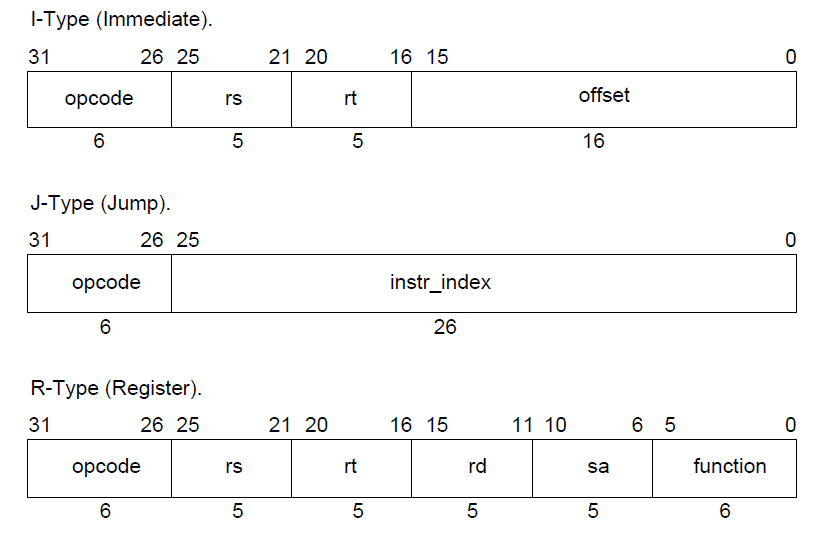
\includegraphics[width=\textwidth]{formats.png}
\end{center}
\caption{MIPS-I instruction formats}
\label{formats}
\end{figure}

In all J-TYPE and I-TYPE instructions 
(except branch instructions comparing one register against zero), 
the opcode field is used to specify instruction type. This class
of instructions is called `instructions encoded by opcode field'.
All possible values for opcode field under this class are shown
in figure \ref{encoding1}, along with valid mnemonics.\\

\begin{figure}[H]
\begin{center}
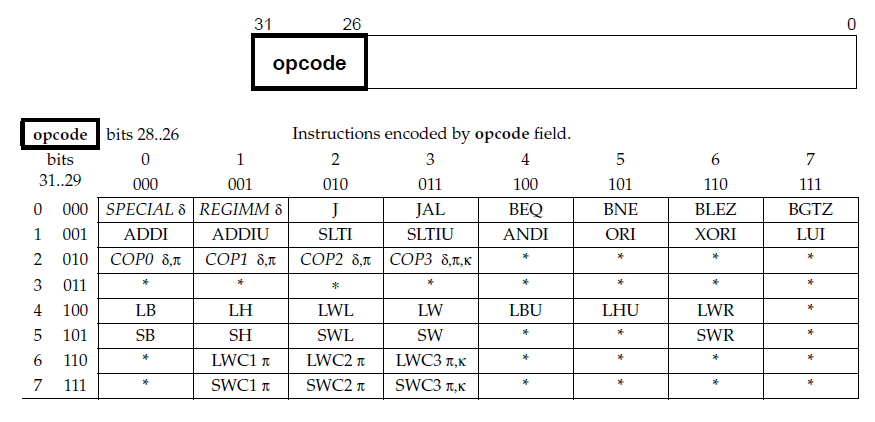
\includegraphics[width=\textwidth]{encoding1.png}
\end{center}
\caption{Instructions encoded by opcode field}
\label{encoding1}
\end{figure}

All R-TYPE instructions (including control instructions)
are encoded using funct field, where opcode field is constant.
For control instructions, the opcode field is equal to $COP0$ constant,
while opcode field of remaining instruction is equal to $SPECIAL$ constant.
R-TYPE instructions with opcode equal to $SPECIAL$ constant form
another third class, called `instructions encoded by function field
when opcode field = $SPECIAL$'. Figure \ref{encoding2} shows
members of this class.\\

\begin{figure}[H]
\begin{center}
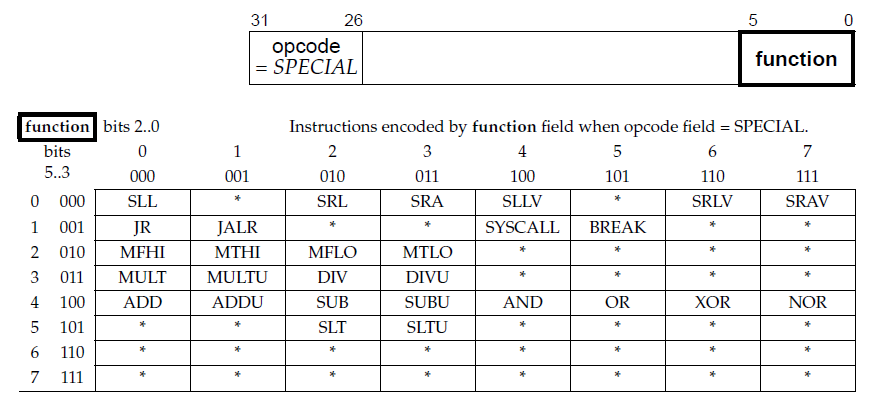
\includegraphics[width=\textwidth]{encoding2.png}
\end{center}
\caption{Instructions encoded by function field when opcode field = $SPECIAL$}
\label{encoding2}
\end{figure}

Finally, branch instructions comparing one register against zero are
encoded using rt field, while opcode field hold a constant value
equal to $REGIMM$ constant (register-immediate).
This class, shown in figure \ref{encoding3}, is called `instructions 
encoded by the rt field when opcode field = $REGIMM$'.\\

\begin{figure}[H]
\begin{center}
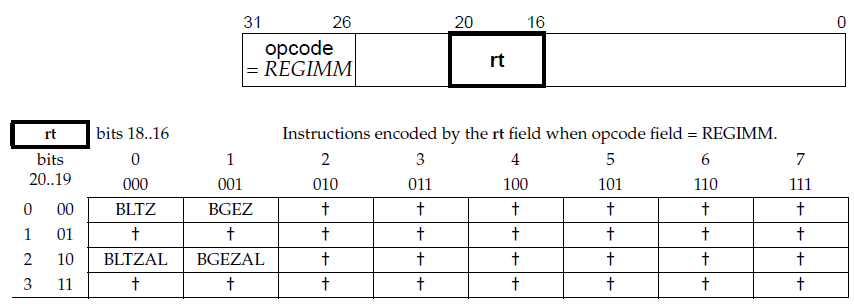
\includegraphics[width=\textwidth]{encoding3.png}
\end{center}
\caption{Instructions encoded by rt field when opcode = $REGIMM$}
\label{encoding3}
\end{figure}

\subsubsection{Addressing Modes}

Figure \ref{addrmodes} summarizes all possible addressing modes 
along with instructions that support them:

\begin{figure}[h]
\begin{center}
\resizebox{0.9\textwidth}{!} {
\begin{tabular}{|c|c|}

\hline \textbf{Addressing Mode} & 
       \textbf{Corresponding Instructions} \\

\hline Register, [Base Register]+Immediate Offset & 
       Load/Store Instructions \\

\hline Register, Register, Immediate & 
       ALU Instructions with Immediate Operand \\

\hline \multirow{2}{*}{Register, Register, Register} &
       ALU Instructions with Three Operands \\
\cline{2-2} & SLLV, SRLV, and SRA \\

\hline Register, Register, Shift Amount &
       SLL, SRL, and SRA \\

\hline Register, Register &
       MULT, MULTU, DIV, and DIVU \\

\hline Register &
       MFHI, MTHI, MFLO, and MTLO \\   

\hline Absolute Address Within 256MB Segment &
       Jump Instructions Jumping Within 256MB Region \\

\hline Register Absolute &
       Jump Instructions to Absolute Address \\

\hline Register, Register, PC-Relative Immediate &
       Branch Instructions Comparing 2 Registers \\

\hline Register, PC-Relative Immediate &
       Branch Instructions Comparing Against Zero \\

\hline Immediate Code &
       Exception Instructions \\

\hline Register, Control Register &
       MFC0 and MTC0 \\

\hline Implicit &
       TLBR, TLBWI, and RFE \\

\hline

\end{tabular}
}
\end{center}
\caption{All possible addressing modes}
\label{addrmodes}
\end{figure}

We note that every instruction has no more than one single addressing
mode, thus MIPS doesn't need an addressing mode field in instruction
word.

\subsubsection{Programmer-Visible Pipeline Effects}

Several effects related to the behaviour of the pipeline should be stated 
clearly so the programmer can be aware of the exact performance parameters
of the running program:

\begin{itemize}

\item \textbf{Delayed branching}: Since the effective address is not available
      immediately after fetching a jump/branch instruction, a delay
      slot should be inserted after the jump/branch instruction. The
      delay instruction is always fetched and executed after the
      jump/branch instruction. The effective address becomes ready
      after fetching the delay instruction and next instruction
      would be the instruction at the new PC.

\item \textbf{Load data not available}: If a memory load instruction is
      followed by an ALU instruction that requires the data
      acquired by the load instruction (addresses the same 
      register), a data hazard will occur since ALU must wait
      until MEM unit is done fetching data from memory. This
      shall delay the execution of the ALU instruction by
      one delay slot (stalls the pipeline for one slot).

\item \textbf{Consequent control instructions}: A control instruction
      may stall if there is another control instruction
      in the pipeline, to prevent data hazards and simultaneous
      access to TLB and stuff.

\item \textbf{Branch instruction operands not ready}:
      If a branch instruction depends on result of the previous
      instruction (or second previous instruction), the pipeline
      will stall until data is ready.

\item \textbf{Multiply/divide instructions}: These four special 
      instructions take more than one CPU clock cycle to complete, 
      therefore they might stall the pipeline.

\item \textbf{Cache misses}: 
      The pipeline shall stall if the instruction to
      be fetched or data specified by load instruction is not in cache.
      Furthermore, store instructions would always stall the pipeline 
      since the cache system is write-through. This means that an
      instruction will take more than one CPU clock cycle if a cache
      miss happens.

\item \textbf{Unaligned memory access}: 
      This class of instructions shall take
      more than one CPU clock cycles because atomic access to unaligned
      word is not possible.

\end{itemize}

Other than the cases specified above, the pipeline will have no 
hazards/stalls and every instruction will take no more than one clock cycle
delay.

\subsection{Registers}
\subsection{Exception Handling}
\subsection{Paging}
\subsection{Cache Management}
\subsection{VHDL Implementation: Introduction}
\subsection{VHDL Implementation: The Pipeline}
\subsection{VHDL Implementation: Exceptions}
\subsection{VHDL Implementation: Cache and TLB}

\end{document}
